% Figure 2 — SSCI computational toolchain architecture (Section 3.5).
% Standalone TikZ; compiles to a cropped PDF with pdflatex, and can also be
% \input into main.tex inside a figure environment.
\documentclass[border=4pt]{standalone}
\usepackage{tikz}
\usepackage{amsmath}
\usepackage{xcolor}
\definecolor{okorange}{RGB}{230,159,0}
\definecolor{oksky}{RGB}{86,180,233}
\definecolor{okblue}{RGB}{0,114,178}
\usetikzlibrary{positioning,arrows.meta,fit,backgrounds,calc}
\begin{document}
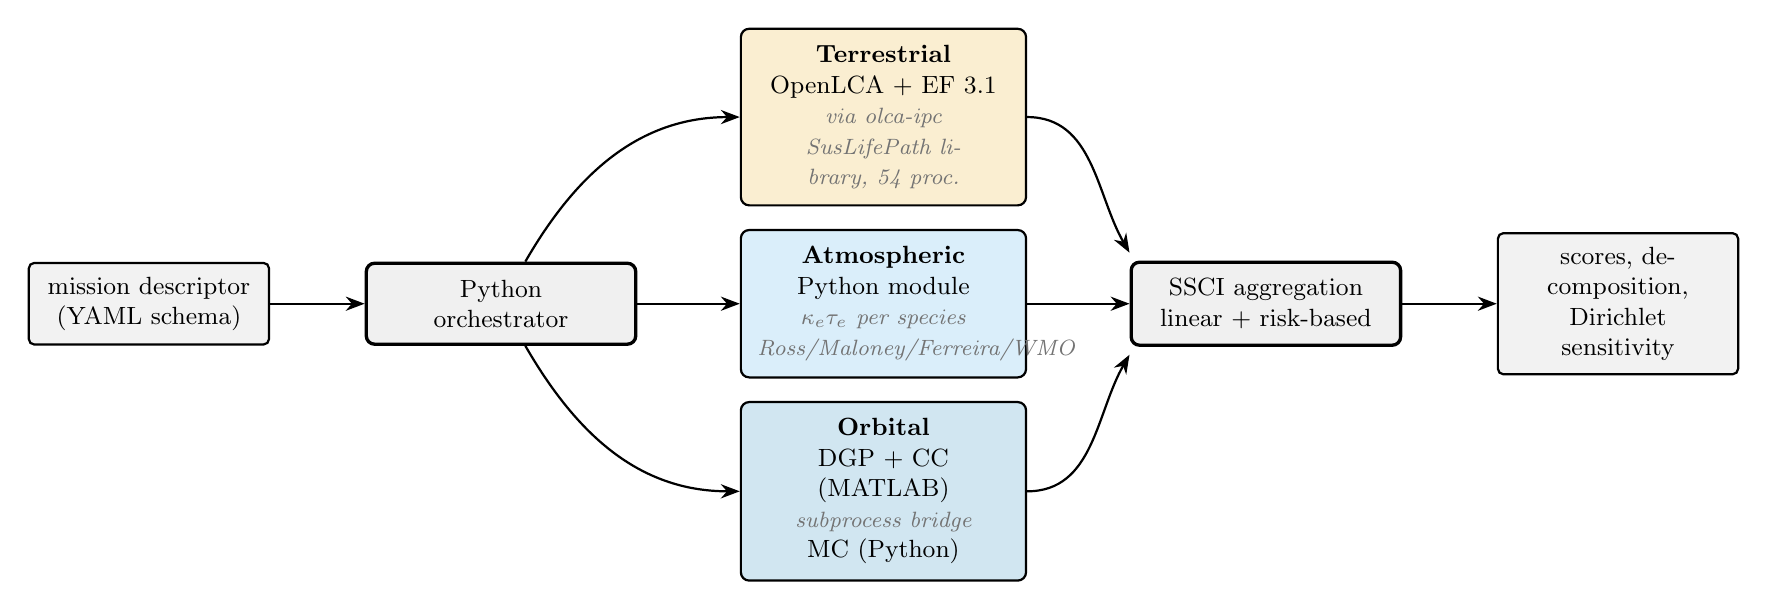
\begin{tikzpicture}[
  font=\small,
  io/.style={rounded corners=2pt, draw, thick, align=center, inner sep=5pt,
             text width=2.7cm, fill=black!5},
  mod/.style={rounded corners=3pt, draw, thick, align=center, inner sep=6pt,
              text width=3.2cm, minimum height=1.7cm},
  orch/.style={rounded corners=3pt, draw, very thick, align=center,
               inner sep=6pt, text width=3.0cm, fill=black!6},
  flow/.style={-{Stealth[length=2.4mm]}, thick},
]

% --- input ---
\node[io] (yaml) {mission descriptor\\ (YAML schema)};

% --- orchestrator ---
\node[orch, right=1.2cm of yaml] (orch) {Python\\ orchestrator};

% --- three domain modules ---
\node[mod, fill=okorange!18,
      above right=0.7cm and 1.3cm of orch] (T) {%
  \textbf{Terrestrial}\\ OpenLCA + EF 3.1\\ {\footnotesize\itshape\color{black!55} via olca-ipc}\\
  {\footnotesize\itshape\color{black!55} SusLifePath library, 54 proc.}};
\node[mod, fill=oksky!22, right=1.3cm of orch] (A) {%
  \textbf{Atmospheric}\\ Python module\\ {\footnotesize\itshape\color{black!55} $\kappa_e\tau_e$ per species}\\
  {\footnotesize\itshape\color{black!55} Ross/Maloney/Ferreira/WMO}};
\node[mod, fill=okblue!18,
      below right=0.7cm and 1.3cm of orch] (O) {%
  \textbf{Orbital}\\ DGP + CC (MATLAB)\\ {\footnotesize\itshape\color{black!55} subprocess bridge}\\
  MC (Python)};

% --- aggregation ---
\node[orch, right=1.3cm of A] (agg) {SSCI aggregation\\ linear + risk-based};

% --- outputs ---
\node[io, right=1.2cm of agg] (out) {scores, decomposition,\\ Dirichlet sensitivity};

% --- flows ---
\draw[flow] (yaml) -- (orch);
\draw[flow] (orch) to[out=60,in=180] (T.west);
\draw[flow] (orch) -- (A.west);
\draw[flow] (orch) to[out=-60,in=180] (O.west);
\draw[flow] (T.east) to[out=0,in=120] ($(agg.north west)+(0,0.1)$);
\draw[flow] (A.east) -- (agg.west);
\draw[flow] (O.east) to[out=0,in=-120] ($(agg.south west)+(0,-0.1)$);
\draw[flow] (agg) -- (out);
% (open-toolchain / MIT / Zenodo note lives in the figure caption)
\end{tikzpicture}
\end{document}
